
\section{C-Elegans} 
\label{section:c-elegans} 

Caenorhabditis elegans (pron.: /ˌseɪnɵræbˈdɪtɪs ˈɛlɛɡænz/) is a free-living, transparent nematode (roundworm).

\begin{itemize}
  \item Size: about 1mm in length
  \item Number of neurons: 
    It is one of the simplest organisms with a nervous system. In the hermaphrodite, this comprises 302 neurons whose pattern of connectivity, or "connectome", has been
    completely mapped and shown to be a \href{http://en.wikipedia.org/wiki/Small-world-network}{small-world network}.
  \item Number of synapses: 7000
  \item Sex: C-elegans has two sexes: hermaphrodites and males. Sex in C. elegans is based on an X0 sex-determination system.

  {\tt http://worms.aecom.yu.edu/}
\end{itemize}

\subsection{Clustering}
To perform natural computation efficiently: specialized modules with locally dense connections

\paragraph{Significance} of the existence of clusters: organization of functional modules.Ganglion vs. synaptic connection;
Topological nature of the structure plays an important role in the information processing of C-elegans network.

\paragraph{C-elegans wiring}
5 anatomical clusters in the C-elegans eonnectome, which correspond to experimentally-identified functional circuits.
cooperation including mechanosensation, chemosensation and navigation

\subsubsection{complex network analysis}
Brain: small-world topology from microscopic level (eg. that of C-elegans)
Scale-free degree distribution
structural and functional motifs
Robustness and fragility of brain structural networks with respect to lesions and diseases

Determination and characterization of hierarchical sluster structure: densely connected groups of nodes with sparser connections among groups
Topological clusters in brain structure may correspond to sets of distinct anatomical modeules of neurons.

\subsubsection{method} 
Modularity-based community detection algorithm for directed weighted networks. (modularity maximizatio approach)
\paragraph{Modularity}
is a quantitative measure defined as the number of edges falling within groups minus the expected number in an equivalent network with edges placed at random.
The modularity value $Q$, indicates the degree to which a given paritition maximizes intra-cluster weights and minimizes inter-cluster weights. Define:
$Q=\frac{1}{4W} s^{T}(B + B^{T})s,$ \\
$B_{ij} = A_{ij} - \frac{S_i^{in} S_j^{out}}{W} $ \\
$B_{ij}$: the extent to which the connections from j to i are prominent. \\
$W = \sum_{ij} A_{ij} = \sum_i S_i^{in} = \sum_i S_i^{out}$
\\
Postive values demonstrate the possible presence of cluster structure.

\paragraph{Complexity}:
 NP-complete; approximation heuristics to obtain a near-optimal community assignment vector.
Constraints for C-elegans: information given by bilateral functional symmetry of the neuron cells.
Simulated annealing method: a generic probabillistic metaheuristic for the global optimization problem of locating a good approximation to the global optimum of a given
function in a large search space.

Prior knowledge: to reduce the number of community assignment vectors
bilateral nuronal pairs have similar functional roles, accepting the principle of structure-function association in evolutionary biology.

Spectral detection; fast unfolding.

\subsubsection{graph model}
Degree: number of synaptic partner neurons of a neuron
Weight: appropriate sum of synapses between specific neuronal partners
Strength: total weights of synaptic connections afferent to or eferent from a neuron.

\subsubsection{result}
\begin{quote}{While C. elegans
neurons are spatially concentrated in a manner related to their
ganglionic affiliation, we failed to observe a strong spatial
localization of neurons belonging to the same cluster, except for
those in clusters 11 and 12.}
\end{quote}

\paragraph{Hierarchical relationship}
of clusters is shown from the reordered adjacency matrix of C-elegans connectome.

\paragraph{Index of Qualitative Variation} measures the diversity of types of ganglia in one cluster. 4 of 5 clusters did not display dominant neurotransmitter type.
Low level of correlation between ganglia and cluster assignment.

\paragraph{Functional Cartography}
\begin{itemize}
  \item within-module weight
  \item participation coefficient
\end{itemize}
Characterize each neuron as either provincial or peripheral node, a hub, or a node with few within-module degrees. The types of nodes have a correlation with the types
of neurons.

\paragraph{Use in Complex Behaviors}
Hub Cluster: outward synapses to clusters having many inward synapses;
authoritative clusters have inward synapses from clusters that bridge to them through outward synapses.

\begin{quote}{Thus, the body-spanning cluster 22, whose members are
predominantly motor neurons, acted as an ‘authority’ receiving
information from hub clusters to produce consequential behaviors.}
\end{quote}

\begin{quote}{the structural clusters indentified in
this study appear to serve as a cohesive sub-module for
information processing at various stages.}
\end{quote}

\subsubsection{Present Constraints}
\begin{itemize}
  \item The lack of more appropriate model about inhibitory / excitatory sysnapses (some paper makes rough guess of the signs of synapses based on neurotransmitter gene
expression data.)
  \item Directionality for gap junctions (even if it existed) cannot be extracted from electron micrographs.
  \item When a presynaptic terminal makes contact with two adjacent processes of different neurons, it is not known which of these processes acts as a postsynaptic
terminal; both might be involved.
\end{itemize}

\subsubsection{Ref}
\url{web.mit.edu/lrv/www/elegans/}  provides information about algorithmic approach to analyzing C-elegans neuronal network data.
\url{www.wormatlas.org/ver1/MoW_built0.92/toc.html}  structure of the nervous system of C-elegans

\subsection{Spectral Analysis of C-elegans}
\label{section: Spectral Analysis}

\paragraph{Note}
There are 4 types of membrane regenerative potentials:
\begin{itemize}
  \item Action potential
  \item Graded potential
  \item Intrinsic oscillation
  \item Plateau potential
\end{itemize}

The following papers disagree on the type of membrane potential that the neurons of C. elegans use: 
\cite{mellem_action_2008}, \cite{lockery_first_2009}, \cite{lockery_quest_2009}.
The last two articles are written by the same people: Shawn Lockery (University of Oregon) and Miriam Goodman (Stanford University).

\paragraph{Hodgkin-Huxley Equation} is used to predict the quantitative behavior of a model nerve under a variety of conditions which corresponded to those in actual
experiments. Their experiments show that the neuron cell membrane potential during an acitivity will rise from $-65mV$ to above $+40mV$ at the peak. This phenonmenon is
explained by the changing permeability of different ions according to their voltage clamp experiment, which turns out to be an accurate electric model of neuron
communication. 

\begin{figure}[h!]
  \centering
  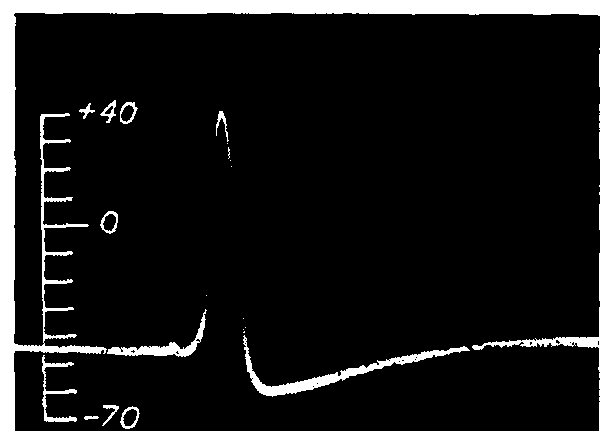
\includegraphics[width=0.5\textwidth]{graphics/ActionPotential}
  \label{fig:action_potential}
  \caption{Action potential and resting potential recorded between inside and outside of axon with capillary filled with sea water. The sea water outside is treated as
zero potential  \cite{Hodgkin_quantitative_1990} }
\end{figure}

% picture from http://www.helcohi.com/sse/body/nervous.html
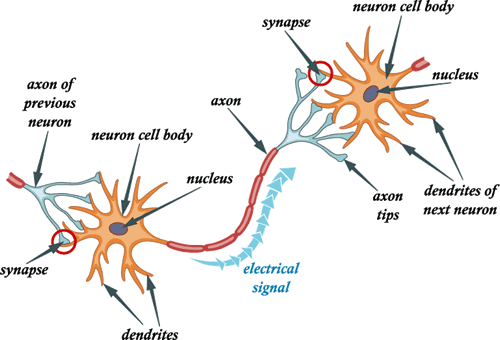
\includegraphics[scale=0.8]{graphics/NeuronSignal}

The following is my summery for the phases that the excitation of neurons goes through:
\begin{enumerate}
  \item The firing threshold is reached. Action potential jumps high. There is influx of sodium ion through the ion channel.
  \item $Na^{+}$ ion causes the membrane to be positively charged. Potassium ion starts to leave the cell(inhibitory factor).
  \item Reaches peak in action potential. Sodium channels becomes refractory, and no more sodium ion is allowed to enter.
  \item Repolarizing phase, when sodium ion channel still in its refractory phase, while potassium ions continues to leave the cell.
  \item Potassium channels close. Sodium channel ends the refractory phase and reset to resting state.
  \item Diffusion of extracellular potassium from cell causes in very slight increase in membrane voltage. (before resting, the cell is in 
	\textbf{hyper-polarizing state}, the cell is not available for the next stimulation.
\end{enumerate}

An illustration of various phases:

% from http://en.wikipedia.org/wiki/Refractory_period_(physiology)
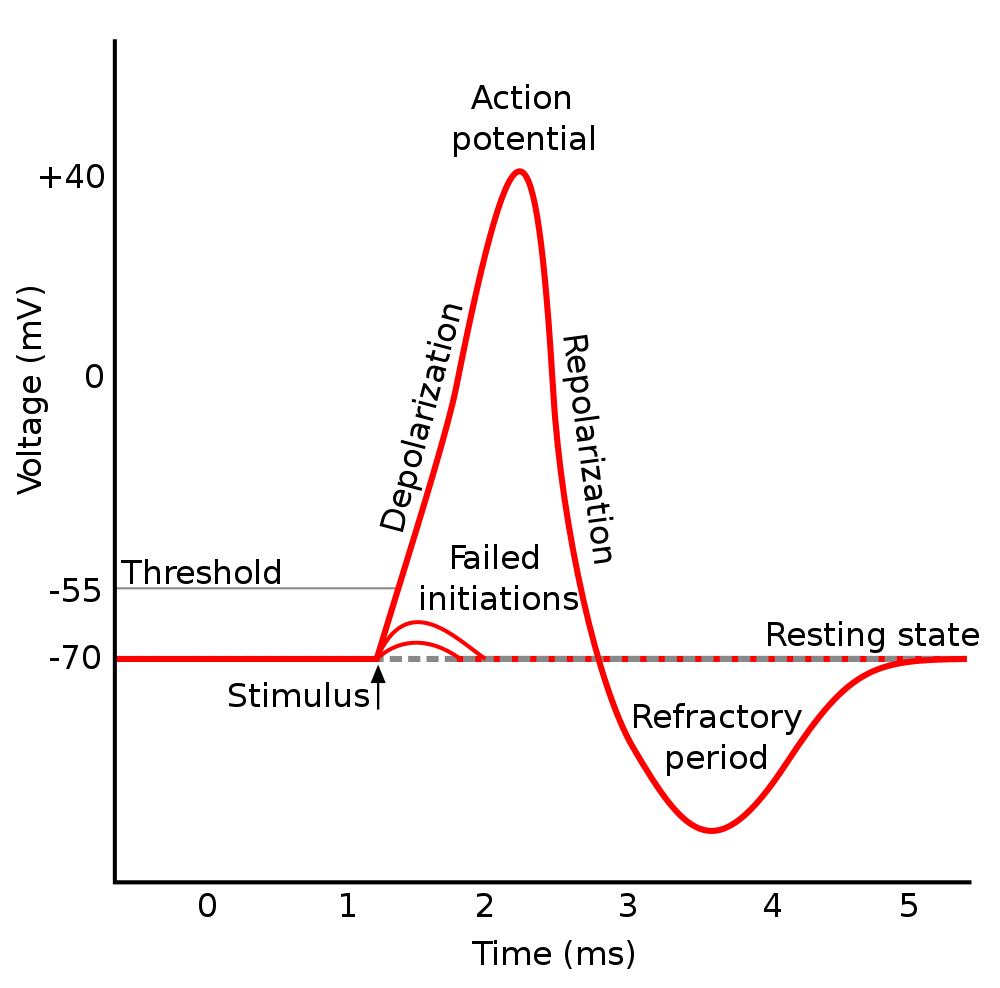
\includegraphics[scale=0.3]{graphics/ActionPotential2}

\subsubsection{Mathematical model}

\paragraph{Model for single cell:}
$$ C_m \frac{dV_m}{dt} + I_{ion} = I. $$
Where $C_m$ denotes membrane capacitance per unit area; $V_m$ the displacement of the membrane potential from its resting value (depolarization
negative); $t$ the time, $I_{ion}$ the net ion current flowing accross the
membrane (inward current positive), and $I$ the total ion current density (inward current positive).

The $I_{ion}$ can be further split into 3 components:
$$ I_{ion} = I_{Na} + I_{K} + I_{l}, \\
\begin{cases}
  I_{Na} = g_{Na} (E - E_{Na}), \\
  I_{K} = g_{K} (E - E_{K}), \\
  I_{l} = {\bar{g}}_{l}.
\end{cases}
$$
The leakage current $I_{l}$ is caused by other ions such as $Cl^{-}$.
$E_{Na}$ and $E_{K}$ are the equilibrium potentials for $Na^{+}$ and $K^{+}$.

The movement of ions is proportional to conductance times driving force.
Let
$$
\begin{cases}
  V = E - E_r, \\
  V_{Na} = E_{Na} - E_r, \\
  V_{K} = E_{K} - E_r, \\
  V_{l} = E_{l} - E_r.
\end{cases}
$$
The $E$s can be replaced by $V$s with respect to resting potential.

Ion channels for different ions contains many gates. If all gates are in permissive state, the channel is considered to be open, and ions are able to go through. The
probability of a gate being in permissive state depends on the current value of the membrane voltage. HH model the gates as their probability of being in permissive
state, ie. $m$, $n$, and $h$. The model specifies the number of gates each ion channel has:

$$
I_{ion} = {\bar{g}}_{Na} m^3 h (V - V_{Na}) + {\bar{g}}_K n^4 (V - V_K) + {\bar{g}}_l (V - Vl),
$$

where
$$ \frac{dn}{dt} = \alpha_n (1 - n) - \beta_n n, $$
$$ \frac{dm}{dt} = \alpha_m (1 - m) - \beta_m m, $$
$$ \frac{dh}{dt} = \alpha_h (1 - h) - \beta_h h. $$

and

$$ \alpha_n = \frac{0.01(V + 10)}{exp \frac{V + 10}{10} - 1}, $$
$$ \beta_n = 0.125 exp \frac{V}{80}, $$
$$ \alpha_m = \frac{0.1(V + 25)}{exp \frac{V + 25}{10} - 1}, $$
$$ \beta_m = 4 exp \frac{V}{18}, $$
$$ \alpha_h = 0.07 exp \frac{V}{20} $$
$$ \beta_h = \frac{1}{exp \frac{V + 30}{10} + 1}. $$

The above number and type of gates for each channel was determined using a trial-and-error method to find the order of gates to achieve the sigmoidal conductance found
from previous results. The best match is the power of 4. The rate constants are obtained by fitting conductance data:

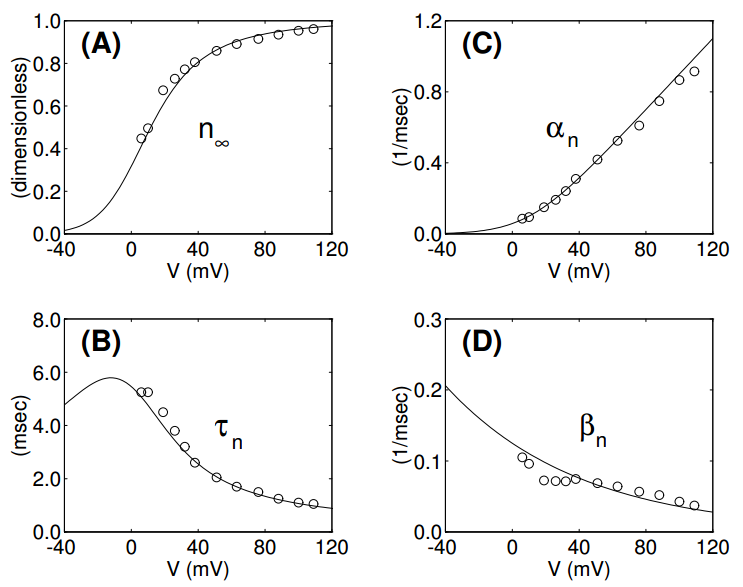
\includegraphics[scale=0.6]{graphics/RateConstants}

\subsubsection{Simplification of HH Equation}
FitzHugh-Nagumo Model:
$$ \dot{V} = V - \frac{V^3}{3} - W + I $$
$$ \dot{W} = 0.08(V + 0.7 - 0.8W) $$





\subsection{Touch Circuit of C. elegans}
\label{section: touch-circuit}

Any such kind of complete circuit would consists of neurons from all 3 categories: sensory neuron, inter-neuron and motor neuron in order to facilitate an observable and
meaningful behavior.

The touch circuit is identified in Chalfie et al. \cite{chalfie_neural_1985}, using laser ablation techniques to kill the precursors of the neuron cells (mostly in
embryos except AVM) and observe its effect on the touch sensitivity of C. elegans.

\subsubsection{Classification}
\paragraph{Sensory input}
There are 6 touch receptor cells:
\begin{itemize}
  \item \emph{ALMR, ALML}: anterior lateral microtubule cells. They are required for a full response to touch on the head.
  \item \emph{PLMR, PLML}: posterior lateral microtubule cells. They are required for any response to touch on the tail.
  \item \emph{AVM}: anterior ventral microtubule cell. AVM alone mediates a very weak touch response to head touch.
  \item \emph{PVM}: posterior ventral microtubule cell. PVM alone does not mediate a detectable touch response.
\end{itemize}

\paragraph{Motor output} 
Sets (coupled by gap junctions) of ventral cord motor neurons are responsible for muscle cell activity: \cite{white_structure_1986}
\begin{itemize}
  \item \emph{A motor neurons} (12 VA cells and 9 DA cells)
  \item \emph{B motor neurons} (11 VBs and 7 DBs)
  \item \emph{D motor neurons} (13 VDs and 6 DDs)
  \item \emph{11 AS motor neurons} share many of the properties of the DA cells
\end{itemize}
A and B neuron cells mediate muscle contraction for backward and forward movement (excitatory), and D cells mediate contralateral inhibition.

From Chalfie et al. \cite{chalfie_neural_1985}, but there is no mention of whether all the A, B, D, AS neurons involve in touch response behavior.

\subsubsection{Data}
From the synapsis data, only 4 pairs of interneurons AVA, AVB, PVC, AVD synapse onto the motor neurons of the ventral cord and span the full length of the cord. They form synapses with touch
cells in an interestingly complementary pattern:

\begin{tabular}{| l | l l |}
  \hline
  \multirow{2}{*}{Interneurons} & \multicolumn{2}{| c |}{Synapses made by} \\ \cline{2-3}
    & Anterior touch receptors & Posterior touch receptors \\ \hline
  AVA & - & chemical \\
  AVB & chemical(only AVM) & - \\
  PVC & chemical & gap \\
  AVD & gap & chemical \\
  \hline
\end{tabular}


\subsubsection{Testing}

\paragraph{Speculation} Is there a relationship between the multiplicity and type of synapses and the effectiveness of that neuron pathway.

Example (Chalfie et al. Figure 4):

The figure below shows that the anterior touch cells (ALM \footnote{AVM not developed in young larvae with which this experiment is carried out}) make EJ with AVA and
AVD, and CJ with PVC; posterior touch cells (PLM) make EJ with PVC, and Chemical with AVD. 
The laser ablation experiment shows that AVA and AVD has no effect on anterior sensitivity, and PVC has no effect on posterior sensitivity. Hence it seems that the gap
junction synapses between sensory and interneurons are more important in this touch circuit.

In contrast, the chemical synapses seem to play an inhibitory role. For example, the Chemical from ALM/AVM to PVC seems to inhibit the neuron signal to be propagated to B
motor neurons, which will cause an inappropriate response.

Data fitting might be able to model the effectiveness of signal propagation in these circuits. In addition to setting a $\tau$ for weight (multiplicity), the type of
synapses could also be taken into account.

Also, lots of connections such as the reciprocal synapses between AVA and PVC are not explained fully in terms of neurology. They might enable/inhibit certain pathways
for certain behavior to be effective. (eg. reaction time)

\paragraph{Rewiring} It seems to me that rewiring could occur as adaptation for C elegans. For C elegans in postembryonic stage, when AVD is killed, they regain some
touch sensitivity after a few more touches, which suggest that the Chemical between AVM-AVB-AVA-AVD \footnote{from experimental results AVA seems to be important in this
alternative pathway} might act as an alternative pathway, which is not the optimum, but might be in
use when the optimum path is damaged.

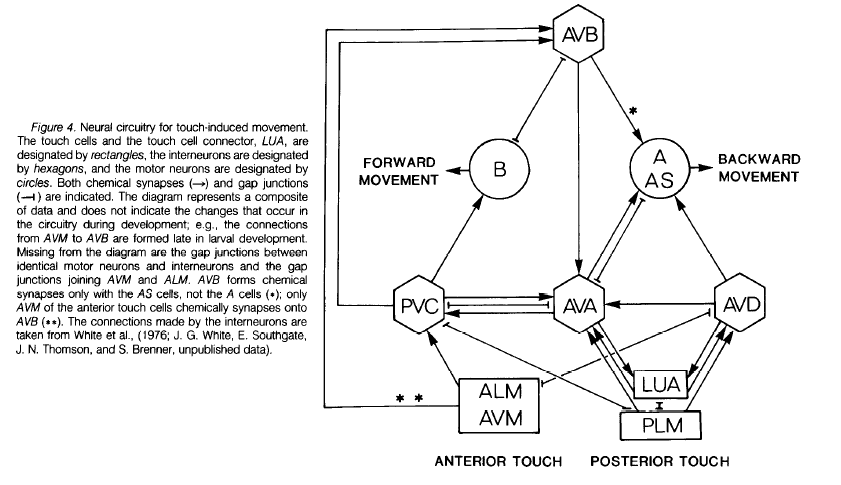
\includegraphics[scale=0.8]{graphics/TouchCircuit}

The following table illustrates the result of disabling certain interneuron(s):

\begin{tabular}{| l | l l l l l l |}
  \hline
  \multirow{2}{*}{Interneurons killed} & \multicolumn{2}{ c }{Sensitive at head} & \multicolumn{2}{ c }{Sensitive at tail}
    & \multirow{2}{*}{Forward movement} & \multirow{2}{*}{Backward movement} \\ \cline{2-3} \cline{4-5}
    & Larva & Adult & Larva & Adult & \\
  PVC & \checkmark & \checkmark & - & - & \checkmark & \checkmark \\
  AVD & - & \checkmark (adapted) & \checkmark & \checkmark & \checkmark & \checkmark \\
  AVD, AVM & - & - & \checkmark & \checkmark & \checkmark & \checkmark \\
  AVA & \checkmark & \checkmark & \checkmark & \checkmark & \checkmark & uncoordinated \footnote{uncoordinated when moving in the indicated direction and when stopping
after moving in the opposite direction} \\
  AVA, AVD & - & \checkmark \footnote{Anterior touch could not make them move backward, but could stop them if they were moving forward. The touch also stopped
pharyngeal pumping} & \checkmark & \checkmark & \checkmark & - \\
  AVB & \checkmark & \checkmark & \checkmark & \checkmark & uncoordinated & \checkmark \\
  AVB, PVC & \checkmark & \checkmark & - & - & - \footnote{incapable of propagating a wave of muscle contraction for forward motion in the body, but did move forward
from waves generated in the head} & \checkmark \\
  \hline
\end{tabular}

\subsection{Other functional circuits suggested}

All these circuits could be the biological ground truth for doing clustering. Checking 1D eigenspace would be simple. 3D needs more thoughts.

\newpage

\begin{figure}[h!]
  \caption{Learned NaCl Aversion. Based on data from Hukema et al.(2006), Tomioka et al. (2006), Fu et al. (2009), Kano et al. (2008), Ishihara et al. (2002), and White et al. (1986)}
  \centering
  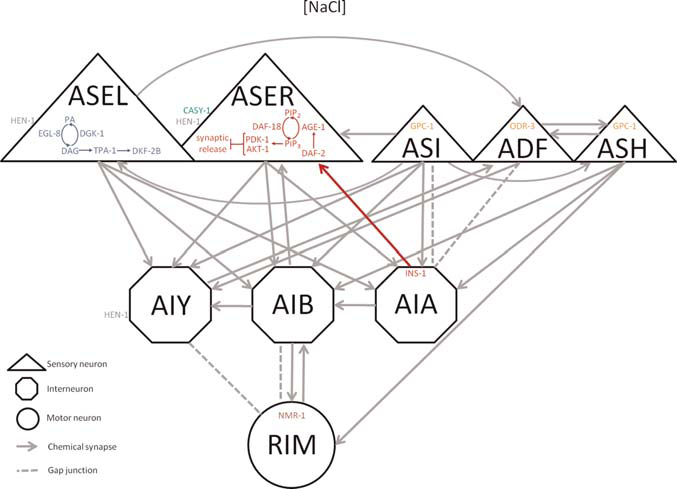
\includegraphics[scale=0.8]{graphics/LearnedNaClAversion}
  \label{fig:NaCl_aversion}
\end{figure}

\begin{figure}[H]
  \paragraph{Electrosensory Behavior \cite{gabel_neural_2007} }
  It is the biological ability to perceive natural electrical stimuli.

  The following diagram is not considered as comprehensive, but the author did suggest why interneurons such as AIY are not significant in electrosensory neural circuits
according to the experiments.

  \centering
  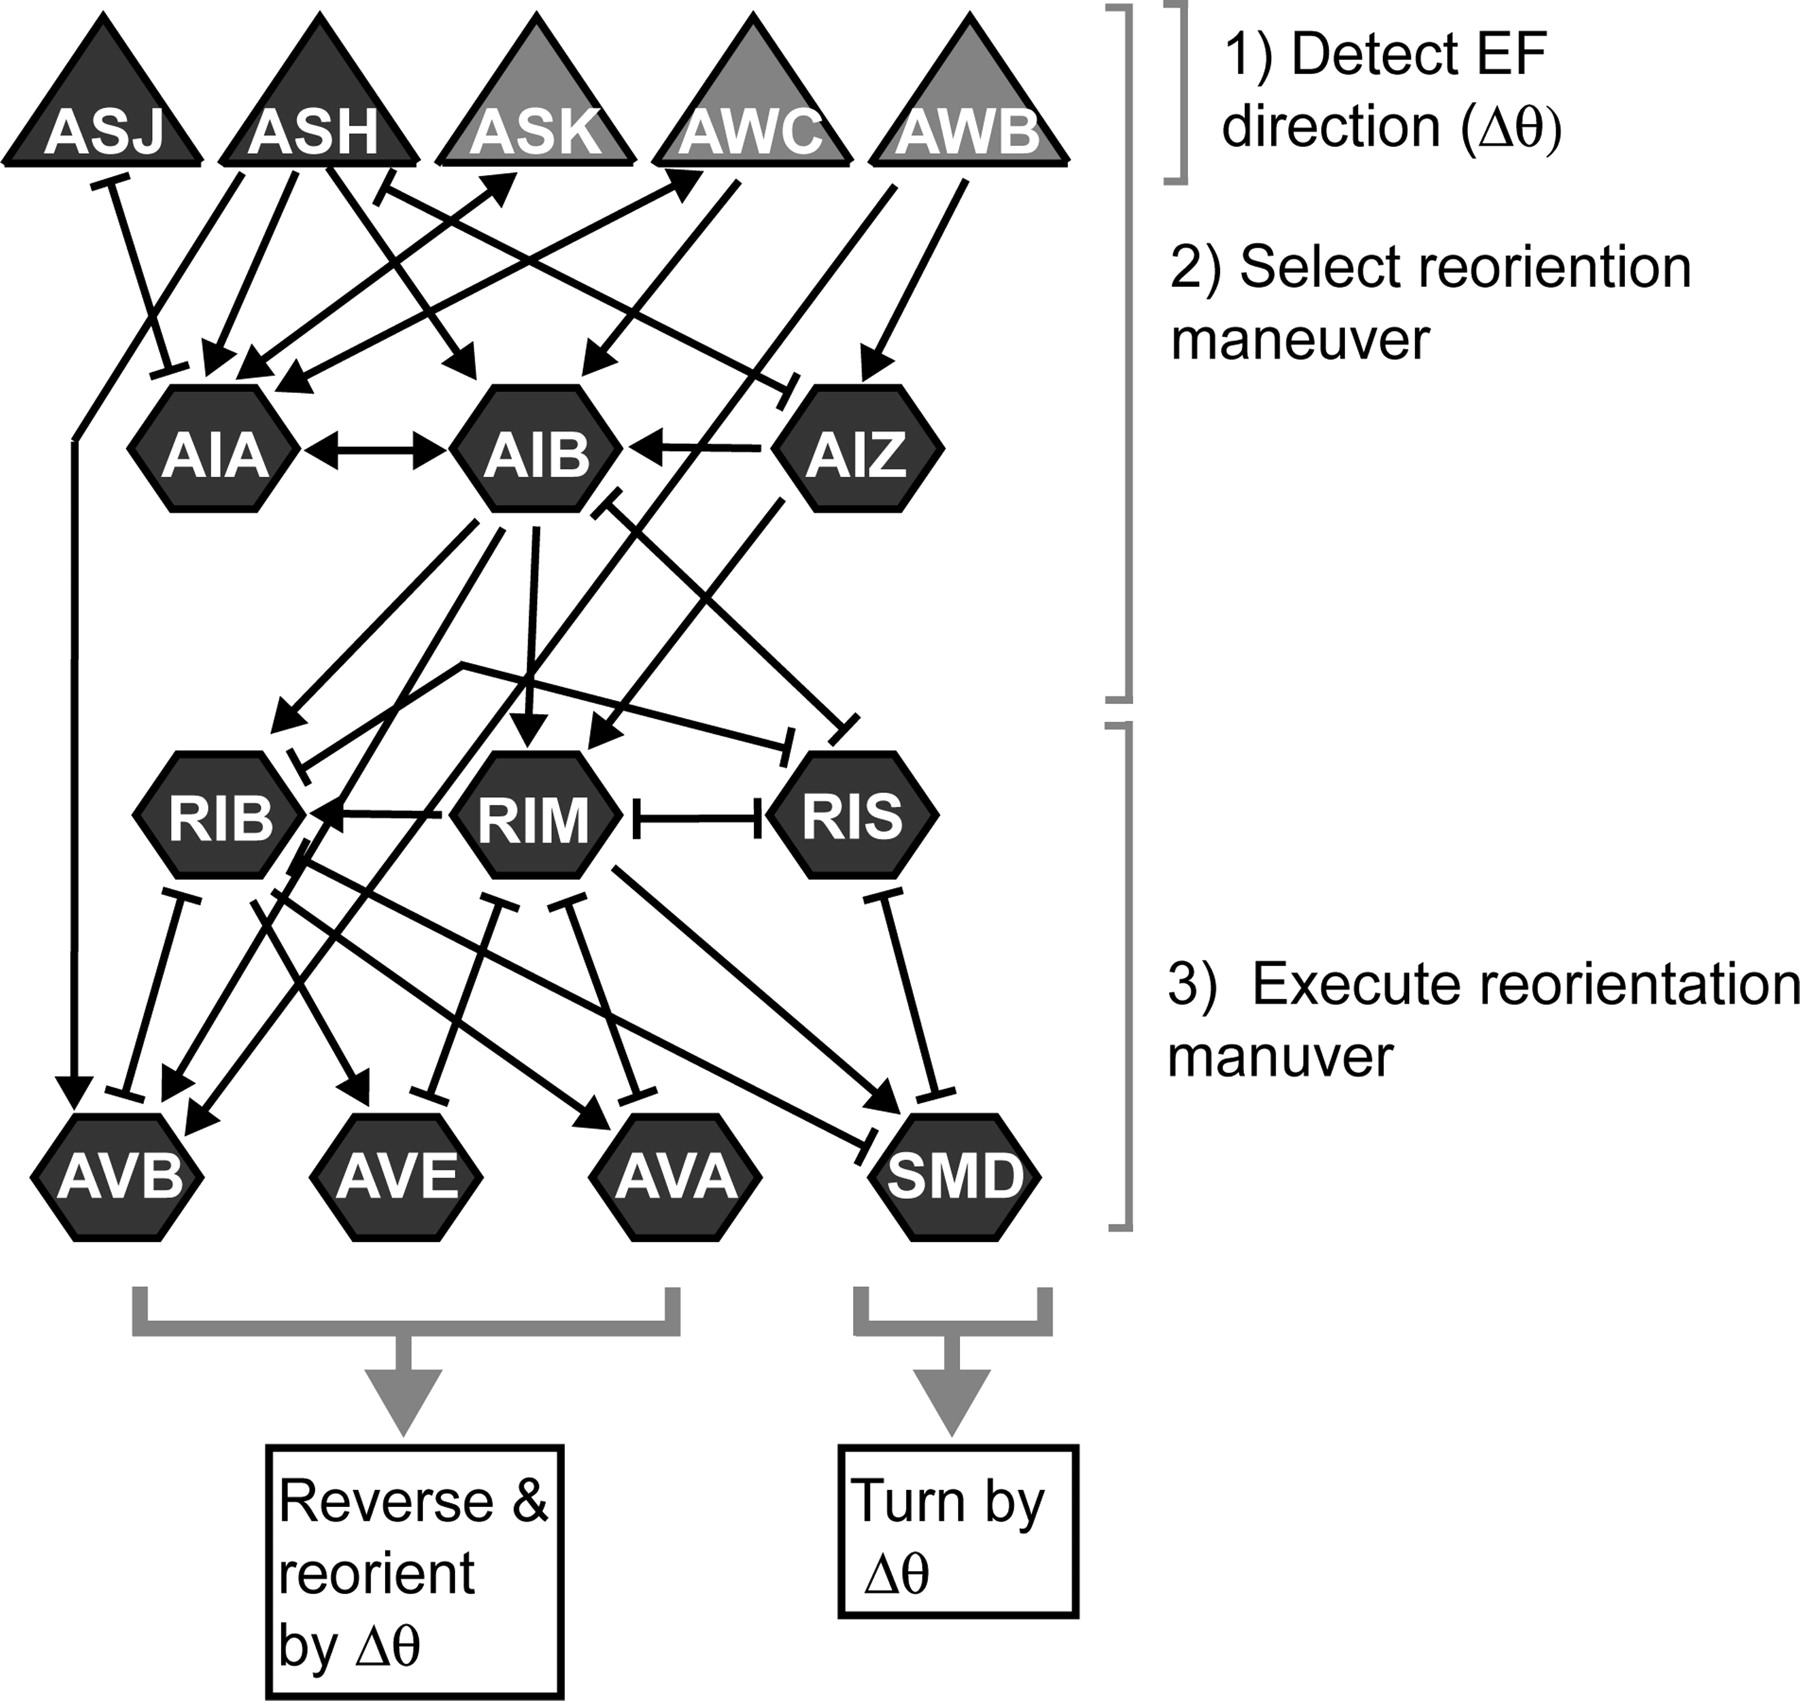
\includegraphics[scale=0.25]{graphics/ElectroSensoryCircuit}
  \label{fig:electro_sensory}
  \caption{Neural circuits for electrosensory behavior. The wiring diagram of neural pathways that might contribute to electrosensory behavior is shown. Synaptic connections
between neurons follow the wiring diagram established by White et al. (1986). Sensory neurons are indicated by red triangles. Interneurons and command motor neurons are
indicated by hexagons. Chemical synaptic connections between neurons are indicated by arrows. Gap junctions are indicated by brackets. We suggest that the primary
neurons for electrosensory detection are ASJ and ASH. RIM and AVA appear contribute to turns and reversals during electrosensory steering, respectively. Additional
neurons show pathways that might connect ASJ, ASH, RIM, and AVA to motor output during electrosensory behavior, as well as several other neurons that have been
implicated in the execution of turns and reversals during exploratory behaviors (Tsalik and Hobert, 2003; Wakabayashi et al., 2004; Gray et al., 2005). EF, Electric
field. sed on data from Hukema et al.(2006), Tomioka et al. (2006), Fu et al. (2009), Kano et al. (2008), Ishihara et al. (2002), and White et al. (1986)}
\end{figure}




\newpage

\subsection{June 18 2013 Work Notes}
\label{06-18-2013}

\newcounter{FigureCounter}
\setcounter{FigureCounter}{1}

Parsing of hermaphrodite C. elegans neuron connection.

\paragraph{Read neuron connect data} from a csv file converted from an excel file "NeuronConnect" downloaded from 2.1 of \url{http://www.wormatlas.org/neuronalwiring.html} (\cite{varshney_structural_2011}). 

script file name: Run\_parseHermConnectome.m.

\paragraph{Figure} \arabcount{FigureCounter}: sparse graph of electric junction visualization.

\paragraph{Figure} \arabcount{FigureCounter} and \arabcount{FigureCounter}: degree/strength plot in descending order. Max degree: 40; max nodal strength: 113.

\paragraph{Figure} \arabcount{FigureCounter}: \Gls{survival-function} for degrees of gap junction network. In real world, there is often noise present at the tail of the
degree distribution: the degree distribution has a long right tail of values that are far above the mean. One method to get arround the problem is to construct a
histogram in which the bin sizes increase exponentially with degree (number of samples in each bin is divided by the width of the bin to normalize measurement); the
other way is to use CDF/survival function (the advantage is there is no loss of information). (in order to check \gls{power-law}).

\paragraph{Figure} \arabcount{FigureCounter}: Histogram of Path Length for Herm Gap Junction Network (weighted). The shortest path computation is done using bioinformatics toolbox
(Johnson Algorithm). Average path length is also calculated.

\paragraph{Other measures}: \Gls{jaccard-coefficient}, \Gls{cluster-coefficient}

\paragraph{Figure} \arabcount{FigureCounter}: sparse graph of Chemical junction visualization.

\subsubsection{Centrality}

Various measures of centrality are used to determine the relative importance of a vertex within the graph.

\paragraph{Degree Centrality} is defined as the number of links incident upon a node. In the case of directed graph, indegree and outdegree centrality values are
calculated. (Definition can be extended to evaluate centrality of graph)

\paragraph{Closeness Centrality} of a node is its total distance to all other nodes. The smaller the value, the more central is the node.

\paragraph{Betweenness Centrality} of a vertex within a graph quantifies the number of times a node acts as a bridge along the shortest path between two other nodes.
Vertices that have a high probability to occur on a randomly chosen shortest path between two randomly chosen vertices have a high betweenness.

$$ C_B(v) = \sum_{s \neq v \neq t \in V} \frac{\sigma_{st} (v)}{\sigma_{st}} $$

Algorithm to compute betweenness of a vertex $v$ in a graph $ G = (V, E) $:
\begin{itemize}
  \item For each pair of vertices $ (s, t) $, compute the shortest path between them
  \item For each pair of vertices $ (s, t) $, determine the fraction of shortest paths that pass through vertex v
  \item Sum this fraction over all pairs of vertices $ (s, t) $
\end{itemize}

\paragraph{Eigenvector Centrality} uses the eigenvector that corresponds to the greatest eigenvector of the adjacency matrix of the graph $x$ to determin the influence
of a node. The score of each node is $ x_i $, based on the concept that connections to high-scoring nodes contribute more to the score of the node in question than equal
connections to low-scoring nodes.




\section{Male C-elegans Wiring Data}
\label{section:male wiring}

Male C. elegans has 81 neurons in addition to hermaphrodite C. Elegans.
\cite{jarrell_connectome_2012}

\paragraph{More info: }
The six most central neurons are: AVAL, AVBR, RIGL, AVBL, RIBL and AVKL

Single combined network by adding the adjacency matrix of the gap junction and chemical networks together:
\begin{quote}
New net work consisting 279 neurons and 2990 directed connections. It has one large strongly connected component of 274 neurons and 5 strongly isolated neurons. The 5
isolated neurons are IL2DL/R, PLNR, DD06, PVDR.
Mean path length $ L = 2.87 $.
\end{quote}

\subsection{Neuron List}
\label{Male (N2Y) Neuron List}

\newpage

\newcounter{ClusterCounter}
\setcounter{ClusterCounter}{1}

%\begin{table}[htbp]
%  \centering
\begin{center}
  \begin{longtable}{ |p{1cm} | p{1.8cm} | p{1.8cm} | p{2.6cm} | p{3.2cm} | p{2.4cm} | p{1.5cm} | p{10cm} |}
    \caption{NEURON LIST, C. ELEGANS ADULT MALE, N2Y SERIES AND CLUSTERING INFORMATION} \tabularnewline
    \toprule
    %\multicolumn{5}{c}{NEURON LIST, C. ELEGANS ADULT MALE, N2Y SERIES} \\
    \midrule
    Index &
    Neurons \footnote{Link to map, synapse lists, circuit diagrams. Standardized: \cite{jarrell_connectome_2012} } & 
    GS/MS \footnote{gender shared (GS) or male-specific (MS)} & 
    Neuron type & 
    Location \footnote{Location of cell body} & 
    Module \footnote{Cluster according to \cite{jarrell_connectome_2012}. There are in total 5 clusters named as: Response, Locomotion, R(1-5)A, PVV, Insemination
Module } &
    Cluster \footnote{Cluster according to \cite{sohn_topological_2011}. There are in total 5 clusters named as: 11, 12, 13, 21, 22 } &
    Notes \\ \hline



% ----------------------------------- Content --------------------------------------------------------------------------
    \arabcount{ClusterCounter} & ADAL & GS & & & & \colorA{11} &  \\
    \arabcount{ClusterCounter} & ADAR & GS & & & & \colorA{11} &  \\
    \arabcount{ClusterCounter} & ADEL & GS & & & & \colorC{13} &  \\
    \arabcount{ClusterCounter} & ADER & GS & & & & \colorC{13} &  \\
    \arabcount{ClusterCounter} & ADFL & GS & & & & \colorA{11} &  \\
    \arabcount{ClusterCounter} & ADFR & GS & & & & \colorA{11} &  \\
    \arabcount{ClusterCounter} & ADLL & GS & & & & \colorA{11} &  \\
    \arabcount{ClusterCounter} & ADLR & GS & & & & \colorA{11} &  \\
    \arabcount{ClusterCounter} & AFDL & GS & & & & \colorA{11} &  \\
    \arabcount{ClusterCounter} & AFDR & GS & & & & \colorA{11} &  \\
    \arabcount{ClusterCounter} & AIAL & GS & & & & \colorA{11} &  \\
    \arabcount{ClusterCounter} & AIAR & GS & & & & \colorA{11} &  \\
    \arabcount{ClusterCounter} & AIBL & GS & & & & \colorA{11} &  \\
    \arabcount{ClusterCounter} & AIBR & GS & & & & \colorA{11} &  \\
    \arabcount{ClusterCounter} & AIML & GS & & & & \colorA{11} &  \\
    \arabcount{ClusterCounter} & AIMR & GS & & & & \colorA{11} &  \\
    \arabcount{ClusterCounter} & AINL & GS & & & & \colorA{11} &  \\
    \arabcount{ClusterCounter} & AINR & GS & & & & \colorA{11} &  \\
    \arabcount{ClusterCounter} & AIYL & GS & & & & \colorA{11} &  \\
    \arabcount{ClusterCounter} & AIYR & GS & & & & \colorA{11} &  \\
    \arabcount{ClusterCounter} & AIZL & GS & & & & \colorA{11} &  \\
    \arabcount{ClusterCounter} & AIZR & GS & & & & \colorA{11} &  \\
    \arabcount{ClusterCounter} & ALA  & GS & & & & \colorB{12} &  \\
    \arabcount{ClusterCounter} & ALML & GS & & & & \colorD{21} &  \\
    \arabcount{ClusterCounter} & ALMR & GS & & & & \colorD{21} &  \\

    \arabcount{ClusterCounter} & ALNL  & GS    & sensory neuron & tail - left lumbar ganglion & N/A & \colorA{11} & 
	Partial reconstruction, few synapses \\
    \arabcount{ClusterCounter} & ALNR  & GS    & sensory neuron & tail - right lumbar ganglion & N/A & \colorA{11} & 
	Partial reconstruction, few synapses \\
    \arabcount{ClusterCounter} & AN1a \footnote{a.k.a. AVFL} & GS    & interneuron & head - lateral / retrovesicular ganglion &  & \colorE{22} & 
	AVF,AVH,AVJ L or R.  Some input in tail \\
    \arabcount{ClusterCounter} & AN1b \footnote{a.k.a. AVFR} & GS    & interneuron & head - lateral / retrovesicular ganglion & & \colorE{22} &
	AVF,AVH,AVJ L or R.  Some input in tail \\
    \arabcount{ClusterCounter} & AN2a \footnote{a.k.a. AVHL} & GS    & interneuron & Head - lateral / retrovesicular ganglion & & \colorE{22} &
	AVF,AVH,AVJ L or R.  Some input/output in tail \\
    \arabcount{ClusterCounter} & AN2b \footnote{a.k.a. AVHR} & GS    & interneuron & head - lateral / retrovesicular ganglion & & \colorE{22} &
	AVF,AVH,AVJ L or R.  Some input/output in tail \\
    \arabcount{ClusterCounter} & AN3a \footnote{a.k.a. AVJL} & GS    & interneuron & head - lateral / retrovesicular ganglion & \colorC{PVV} & \colorD{21} &
	AVF,AVH,AVJ L or R.  Considerable input/output with R1BR \\
    \arabcount{ClusterCounter} & AN3B \footnote{a.k.a. AVJR} & GS    & interneuron & head - lateral / retrovesicular ganglion & \colorC{PVV} & \colorD{21} &
	AVF,AVH,AVJ L or R.  Considerable input/output with R5BR \\

    \arabcount{ClusterCounter} & AQR  & GS & & & & \colorC{13} &  \\
    \arabcount{ClusterCounter} & AS01 & GS & & & & \colorD{21} &  \\
    \arabcount{ClusterCounter} & AS02 & GS & & & & \colorE{22} &  \\
    \arabcount{ClusterCounter} & AS03 & GS & & & & \colorE{22} &  \\
    \arabcount{ClusterCounter} & AS04 & GS & & & & \colorE{22} &  \\
    \arabcount{ClusterCounter} & AS05 & GS & & & & \colorE{22} &  \\
    \arabcount{ClusterCounter} & AS06 & GS & & & & \colorE{22} &  \\

    \arabcount{ClusterCounter} & AS08  & GS    & motor neuron & tail - ventral cord & \colorE{Locomotion} & \colorD{21} &
	Ventral portion only reconstructed. Makes gap junctions with, and postsynaptic to, AVA \\
    \arabcount{ClusterCounter} & AS09  & GS    & motor neuron & tail - ventral cord & \colorE{Locomotion} & \colorD{21} &
	Ventral portion only reconstructed. Makes gap junctions with, and postsynaptic to, AVA \\
    \arabcount{ClusterCounter} & AS10  & GS    & motor neuron & tail - preanal ganglion & \colorE{Locomotion} & \colorD{21} &
	Ventral portion only reconstructed. Makes gap junctions with, and postsynaptic to, AVA \\
    \arabcount{ClusterCounter} & AS11  & GS    & motor neuron & tail - preanal ganglion & \colorC{PVV} & \colorD{21} &
	Postsynaptic to AVA in the ventral cord.  Presynaptic to VD13 and body wall muscles in the dorsal cord \\

    \arabcount{ClusterCounter} & ASEL & GS & & & & \colorA{11} &  \\
    \arabcount{ClusterCounter} & ASER & GS & & & & \colorA{11} &  \\
    \arabcount{ClusterCounter} & ASGL & GS & & & & \colorA{11} &  \\
    \arabcount{ClusterCounter} & ASGR & GS & & & & \colorA{11} &  \\
    \arabcount{ClusterCounter} & ASHL & GS & & & & \colorA{11} &  \\
    \arabcount{ClusterCounter} & ASHR & GS & & & & \colorA{11} &  \\
    \arabcount{ClusterCounter} & ASEL & GS & & & & \colorA{11} &  \\
    \arabcount{ClusterCounter} & ASEL & GS & & & & \colorA{11} &  \\
    \arabcount{ClusterCounter} & ASEL & GS & & & & \colorA{11} &  \\
    \arabcount{ClusterCounter} & ASEL & GS & & & & \colorA{11} &  \\
    \arabcount{ClusterCounter} & ASEL & GS & & & & \colorA{11} &  \\
    \arabcount{ClusterCounter} & ASEL & GS & & & & \colorA{11} &  \\
    \arabcount{ClusterCounter} & ASEL & GS & & & & \colorA{11} &  \\
    \arabcount{ClusterCounter} & ASEL & GS & & & & \colorA{11} &  \\

    \arabcount{ClusterCounter} & AVAL  & GS    & interneuron & head - left lateral ganglion & \colorE{Locomotion} & \colorD{21} &
	Command interneuron, makes gap junctions with A-type body wall motor neurons in the ventral cord. Input from PQR, PVY and PVX, output to A-type motor neurons \\
    \arabcount{ClusterCounter} & AVAR  & GS    & interneuron & head - right lateral ganglion & \colorE{Locomotion} & \colorD{21} &
	Command interneuron, makes gap junctions with A-type body wall motor neurons in the ventral cord. Input from PQR, output to A-type motor neurons \\
    \arabcount{ClusterCounter} & AVBL  & GS    & interneuron & head - left lateral ganglion & \colorE{Locomotion} & \colorD{21} &
	Command interneuron, makes gap junctions with B-type body wall motor neurons in the ventral cord.  Input from AVA \\
    \arabcount{ClusterCounter} & AVBR  & GS    & interneuron & head - right lateral ganglion & \colorD{Response} & \colorD{21} &
	Command interneuron, makes gap junctions with B-type body wall motor neurons in the ventral cord.  Input from MS interneurons \\
    \arabcount{ClusterCounter} & AVDL  & GS    & interneuron & head - left lateral ganglion & \colorE{Locomotion} & \colorD{21} &
	Command interneuron, makes gap junctions with, and presynaptic to, AVA \\
    \arabcount{ClusterCounter} & AVDR  & GS    & interneuron & head - right lateral ganglion & \colorE{Locomotion} & \colorD{21} &
	Command interneuron, makes gap junctions with, and presynaptic to, AVA \\
    \arabcount{ClusterCounter} & AVG   & GS    & interneuron & head - retrovesicular ganglion & \colorD{Response} & \colorD{21} &
	Guidepost interneuron, considerable input from HOA and LUA. \\
    \arabcount{ClusterCounter} & AVKL  & GS    & interneuron & head - left ventral ganglion & & \colorC{13} &
	Makes gap junctions with hypodermis.  Input from PDER \\
    \arabcount{ClusterCounter} & AVKR  & GS    & interneuron & head - right ventral ganglion & & \colorC{13} &
	Runs on left side of preanal ganglion, makes gap junctions with hypodermis and PVS \\
    \arabcount{ClusterCounter} & AVL   & GS    & interneuron & head - right ventral ganglion & \colorA{Insemination} & \colorC{13} &
	Makes gap junctions with PDB, few synapses onto gonad and ventral body wall muscles \\
    \arabcount{ClusterCounter} & CA02  & MS    & interneuron & tail - ventral cord & \colorA{Insemination} & &
	Uncertain cell ID, partial reconstruction \\
    \arabcount{ClusterCounter} & CA03  & MS    & interneuron & tail - ventral cord & \colorA{Insemination} & &
	Uncertain cell ID, partial reconstruction \\
    \arabcount{ClusterCounter} & CA04  & MS    & interneuron & tail - ventral cord & \colorC{PVV} & &
	Uncertain cell ID, extensive branching in the preanal ganglion. Makes many gap junctions with PVV. Input from Ray neurons \\
    \arabcount{ClusterCounter} & CA05  & MS    & interneuron & tail - ventral cord & \colorA{Insemination} & &
	Makes many gap junctions with CA06. Input from MS sensory neurons \\
    \arabcount{ClusterCounter} & CA06  & MS    & interneuron & tail - ventral cord & \colorA{Insemination} & &
	Posteriorly directed process bifurcates posterior to preanal ganglion, with one process running in the left and right cloacal commissures, each.  Makes many gap junctions with CA05. Input from MS sensory neurons.  Process from cell body Enters right side commissure, destination of this process unknown. \\
    \arabcount{ClusterCounter} & CA07  & MS    & interneuron & tail - ventral cord & \colorD{Response} & &
	Process from cell body Enters right side commissure. Unbranched process in preanal ganglion with few synapses \\
    \arabcount{ClusterCounter} & CA08  & MS    & interneuron & tail - preanal ganglion & \colorE{Locomotion} & &
	Process from cell body Enters right side commissure. Anteriorily directed process has few synapses onto gonad and ventral body wall muscle \\
    \arabcount{ClusterCounter} & CA09  & MS    & interneuron & tail - preanal ganglion & \colorB{R(1-5)A} & &
	Extensive branching with very few synapses.  Process from cell body Enters right side commissure, destination of this process unknown. \\
    \arabcount{ClusterCounter} & CP01  & MS    & interneuron & tail - ventral cord & \colorA{Insemination} & &
	Uncertain cell ID. Unbranched process makes many gap junctions with CP02. Considerable output to HOB. \\
    \arabcount{ClusterCounter} & CP02  & MS    & interneuron & tail - ventral cord & \colorA{Insemination} & &
	Uncertain cell ID. Unbranched process makes many gap junctions with CP01. Several synapses onto HOA and HOB \\
    \arabcount{ClusterCounter} & CP03  & MS    & interneuron & tail - ventral cord & \colorA{Insemination} & &
	Uncertain cell ID, unbranched process. Makes NMJs with body wall muscles and anterior inner longitudinal muscles. \\
    \arabcount{ClusterCounter} & CP04  & MS    & interneuron & tail - ventral cord & \colorA{Insemination} & &
	Unbranched process, input from MS sensory neurons. NMJs with body wall muscle \\
    \arabcount{ClusterCounter} & CP05  & MS    & interneuron & tail - ventral cord & \colorA{Insemination} & &
	Innervates the gonad \\
    \arabcount{ClusterCounter} & CP06  & MS    & interneuron & tail - ventral cord & \colorA{Insemination} & &
	Innervates the gonad \\
    \arabcount{ClusterCounter} & CP07  & MS    & interneuron & tail - ventral cord & \colorC{PVV} & &
	Several branches at posterior end. Makes gap junctions with Ray 7 neurons. Multiple inputs and outputs \\
    \arabcount{ClusterCounter} & CP08  & MS    & interneuron & tail - preanal ganglion & \colorC{PVV} & &
	Highly branched at posterior end. Makes gap junctions with Ray 7 neurons. Multiple inputs and outputs \\
    \arabcount{ClusterCounter} & CP09  & MS    & interneuron & tail - preanal ganglion & \colorC{PVV} & &
	Highly branched at posterior end. Makes gap junctions with Ray 6 neurons. Main output to PVV and PDB \\
    \arabcount{ClusterCounter} & DA04  & GS    & motor neuron & tail - ventral cord & \colorD{Response} & \colorE{22} &
	Uncertain cell ID. Partial reconstruction of ventral portion \\
    \arabcount{ClusterCounter} & DA05  & GS    & motor neuron & tail - ventral cord & \colorE{Locomotion} & \colorE{22} &
	Uncertain cell ID. Partial reconstruction of ventral portion \\
    \arabcount{ClusterCounter} & DA06  & GS    & motor neuron & tail - ventral cord & \colorE{Locomotion} & \colorD{21} &
	Ventral portion only reconstructed. Makes gap junctions with, and postsynaptic to, AVA \\
    \arabcount{ClusterCounter} & DA07  & GS    & motor neuron & tail - ventral cord & \colorE{Locomotion} & \colorD{21} &
	Ventral portion only reconstructed. Makes gap junctions with, and postsynaptic to, AVA \\
    \arabcount{ClusterCounter} & DA08  & GS    & motor neuron & tail - ventral cord & \colorE{Locomotion} & \colorD{21} &
	Makes gap junctions with AVA in ventral cord. Presynaptic to D-type motor neurons and body wall muscle in dorsal cord \\
    \arabcount{ClusterCounter} & DA09  & GS    & motor neuron & tail - ventral cord & \colorE{Locomotion} & \colorD{21} &
	Makes gap junctions with AVA and postsynaptic to R1B in ventral cord. NMJs with body wall muscle in dorsal cord \\
    \arabcount{ClusterCounter} & DB03  & GS    & motor neuron & tail - ventral cord & & \colorE{22} &
	Uncertain cell ID. Partial reconstruction of ventral portion \\
    \arabcount{ClusterCounter} & DB04  & GS    & motor neuron & tail - ventral cord & \colorE{Locomotion} & \colorE{22} &
	Uncertain cell ID. Partial reconstruction of ventral portion \\
    \arabcount{ClusterCounter} & DB05  & GS    & motor neuron & tail - ventral cord & \colorE{Locomotion} & \colorD{21} &
	Uncertain cell ID. Partial reconstruction of ventral portion \\
    \arabcount{ClusterCounter} & DB06  & GS    & motor neuron & tail - ventral cord & \colorE{Locomotion} & \colorD{21} &
	Ventral portion only reconstructed. Makes gap junctions with AVB. Input from PQR and A-type motor and interneurons \\
    \arabcount{ClusterCounter} & DB07  & GS    & motor neuron & tail - preanal ganglion & \colorE{Locomotion} & \colorD{21} &
	Ventral portion only reconstructed. Makes gap junctions with AVB. Iinput from VA12 and R9B \\
    \arabcount{ClusterCounter} & DD03  & GS    & motor neuron & tail - ventral cord & \colorE{Locomotion} & \colorE{22} &
	Uncertain cell ID. Partial reconstruction of ventral portion \\
    \arabcount{ClusterCounter} & DD04  & GS    & motor neuron & tail - ventral cord & \colorE{Locomotion} & \colorE{22} &
	Ventral portion only reconstructed. Makes gap junctions with VD motor neuron. Input from VA and VB type motor neurons \\
    \arabcount{ClusterCounter} & DD05  & GS    & motor neuron & tail - ventral cord & \colorE{Locomotion} & \colorE{22} &
	Ventral portion only reconstructed. Makes gap junctions with PVZ and VD motor neurons. Input from VA and VB motor neurons \\
    \arabcount{ClusterCounter} & DD06  & GS    & motor neuron & tail - preanal ganglion & \colorE{Locomotion} & \colorD{21} &
	Ventral cord process has few minor branches. Input from SPV, R2A and VA and VB motor neurons. Dorsal cord process makes NMJs with body wall muscles \\
    \arabcount{ClusterCounter} & DVA   & GS    & interneuron & tail - dorsorectal ganglion & & \colorD{21} &
	Makes gap junctions with AVKL. Input from R1B and postdeirid sensory neurons in ventral cord \\
    \arabcount{ClusterCounter} & DVB   & GS    & interneuron & tail - dorsorectal ganglion & \colorA{Insemination} & \colorD{21} &
	Makes NMJs with ventral spicule protractor muscles \\
    \arabcount{ClusterCounter} & DVC   & GS    & interneuron & tail - dorsorectal ganglion & \colorE{Locomotion} & \colorC{13} &
	Makes gap junctions with DVF. Varied input/output \\
    \arabcount{ClusterCounter} & DVE   & MS    & interneuron & tail - dorsorectal ganglion & \colorA{Insemination} & N/A &
	Presynaptic to EF1 and EF2. Postsynaptic to HOB \\
    \arabcount{ClusterCounter} & DVF   & MS    & interneuron & tail - dorsorectal ganglion & \colorA{Insemination} & N/A &
	Makes gap junctions with SPC. Input from HOB. Output to HOB and SPC \\
    \arabcount{ClusterCounter} & DX1   & MS    & interneuron & tail - dorsorectal ganglion & \colorD{Response} & N/A &
	Makes few gap junctions with dorsal body wall muscles. Input from HOB. Output to PCA in the preanal ganglion \\
    \arabcount{ClusterCounter} & DX2   & MS    & interneuron & tail - dorsorectal ganglion & \colorA{Insemination} & N/A &
	 Makes gap junctions with dorsal body wall muscles. Input from HOB and R3B. Output to PCA in the preanal ganglion \\
    \arabcount{ClusterCounter} & DX3   & MS    & interneuron & tail - dorsorectal ganglion & \colorD{Response} & N/A &
	Makes gap junctions with dorsal body wall muscles. Input from HOB. Output to PCA in the preanal ganglion \\
    \arabcount{ClusterCounter} & EF1   & MS    & interneuron & tail - dorsorectal ganglion & & N/A &
	Forms sheet-like, branchy structure in the preanal ganglion. Makes gap junctions with other EF neurons. Considerable input from RayB neurons. \\
    \arabcount{ClusterCounter} & EF2   & MS    & interneuron & tail - dorsorectal ganglion & &  N/A &
	Forms sheet-like, branchy structure in the preanal ganglion. Makes gap junctions with other EF neurons. Considerable input from RayB neurons. \\
    \arabcount{ClusterCounter} & EF3   & MS    & interneuron & tail - preanal ganglion & & N/A &
	Forms sheet-like, branchy structure in the preanal ganglion. Makes gap junctions with other EF neurons. Considerable input from RayB neurons. \\
    \arabcount{ClusterCounter} & HOA   & MS    & sensory neuron & tail - preanal ganglion & \colorD{Response} & N/A &
	Very large cell body at left posterior end of the preanal ganglion. Makes many gap junctions with PVZ, PCA and PCB.  Presynatptic to LUA, AVG and R8A. Postsynaptic to HOB and LUA \\
    \arabcount{ClusterCounter} & HOB   & MS    & sensory neuron & tail - preanal ganglion & \colorA{Insemination} & N/A &
	Very large cell body at left posterior end of the preanal ganglion. Makes gap junctions with PCB and HOA.  Presynaptic to HOA, PVZ and PCA. Multiple inputs \\
    \arabcount{ClusterCounter} & LUAL  & GS    & interneuron & tail - left lumbar ganglion & \colorD{Response} & \colorD{21} &
	Input from HOA and RayB neurons. Output to AVG and multiple MS neurons. \\
    \arabcount{ClusterCounter} & LUAR  & GS    & interneuron & tail - right lumbar ganglion & \colorD{Response} & \colorD{21} &
	Input from HOA and Ray neurons. Output to AVG and MS interneurons. \\
    \arabcount{ClusterCounter} & PCAL  & MS    & sensory neuron & tail - left cloacal ganglion & \colorD{Response} & N/A &
	Makes gap junctions with HOA. Input from HOB. Output to PVX and R8A. \\
    \arabcount{ClusterCounter} & PCAR  & MS    & sensory neuron & tail - right cloacal ganglion & \colorD{Response} & N/A &
	Makes gap junctions with HOA. Input from HOB. Output to PVX and R8A. \\
    \arabcount{ClusterCounter} & PCBL  & MS    & sensory/motor neuron & tail - left cloacal ganglion & \colorA{Insemination} & N/A &
	Makes NMJs with anterior and posterior oblique muscles. Makes gap junctions with HOA and HOB. Input from PCA \\
    \arabcount{ClusterCounter} & PCBR  & MS    & sensory/motor neuron & tail - right cloacal ganglion & \colorA{Insemination} & N/A & 
	Makes NMJs with anterior and posterior oblique muscles. Makes gap junctions with HOB. Input from PCA \\
    \arabcount{ClusterCounter} & PCCL  & MS    & sensory/motor neuron & tail - left cloacal ganglion & \colorA{Insemination} & N/A &
	Innervates the gonad and the left oblique muscles \\
    \arabcount{ClusterCounter} & PCCR  & MS    & sensory/motor neuron & tail - right cloacal ganglion & & N/A &
	Innervates the gonad and the right posterior oblique muscle \\
    \arabcount{ClusterCounter} & PDA   & GS    & motor neuron & tail - preanal ganglion & \colorC{PVV} & \colorD{21} &
	Makes NMJs with dorsal body wall muscles \\
    \arabcount{ClusterCounter} & PDB   & GS    & interneuron & tail - preanal ganglion & \colorC{PVV} & \colorD{21} &
	Makes NMJs with dorsal body wall muscles. Output to sensory and interneurons. Input from CP07-09. \\
    \arabcount{ClusterCounter} & PDC   & MS    & interneuron & tail - preanal ganglion & \colorC{PVV} & N/A &
	Makes NMJs with dorsal body wall muscles. Makes gap junctions with R5A. Input from Ray 7 neurons \\
    \arabcount{ClusterCounter} & PDEL  & GS    & sensory neuron & posterior half of body - left & & \colorD{21} &
	Input/output with other postdeirid neurons and DVA and AVK in the ventral cord \\
    \arabcount{ClusterCounter} & PDER  & GS    & sensory neuron & posterior half of body - right & & \colorD{21} &
	Input/output with other postdeirid neurons and DVA and AVK in the ventral cord \\
    \arabcount{ClusterCounter} & PGA   & MS    & interneuron & tail - preanal ganglion & \colorC{PVV} & N/A &
	Multiple "weak" inputs/outputs \\
    \arabcount{ClusterCounter} & PHAL  & GS    & sensory neuron & tail - left lumbar ganglion & \colorD{Response} & \colorD{21} &
	Makes gap junctions with other phasmid neurons. Output to EF3, PVX and R3B \\
    \arabcount{ClusterCounter} & PHAR  & GS    & sensory neuron & tail - right lumbar ganglion & \colorD{Response} & \colorD{21} &
	Makes gap junctions with PVQR and other phasmid neurons. Output to R9B and EF1 and EF2 \\
    \arabcount{ClusterCounter} & PHBL  & GS    & sensory neuron & tail - left lumbar ganglion & \colorD{Response} & \colorD{21} &
	Makes gap junctions with PHAL. Input/output with R3B \\
    \arabcount{ClusterCounter} & PHBR  & GS    & sensory neuron & tail - right lumbar ganglion & \colorD{Response} & \colorD{21} &
	Makes gap junctions with PHAR. Output to EF2 and R9B \\
    \arabcount{ClusterCounter} & PHCL  & GS    & sensory neuron & tail - left lumbar ganglion & & \colorD{21} &
	Output to AVA/AVD \\
    \arabcount{ClusterCounter} & PHCR  & GS    & sensory neuron & tail - right lumbar ganglion & & \colorD{21} &
	Output to AVA/AVD \\
    \arabcount{ClusterCounter} & PLML  & GS    & sensory neuron & tail - left lumbar ganglion & & \colorD{21} &
	Ventral cord process makes gap junctions with PVR. Output to PDE \\
    \arabcount{ClusterCounter} & PLMR  & GS    & sensory neuron & tail - right lumbar ganglion & & \colorD{21} &
	Ventral cord process makes gap junctions with PVR. Output to DVA and PDE \\
    \arabcount{ClusterCounter} & PLNL  & GS    & sensory neuron & tail - left lumbar ganglion & & \colorA{11} &
	Some Ray neuron input \\
    \arabcount{ClusterCounter} & PLNR  & GS    & sensory neuron & tail - right lumbar ganglion & & \colorA{11} &
	Some Ray neuron input \\
    \arabcount{ClusterCounter} & PQR   & GS    & sensory neuron & tail - left lumbar ganglion & & \colorD{21} &
	Input from MS sensory neurons. Output to AVA and AVD \\
    \arabcount{ClusterCounter} & PVCL  & GS    & interneuron & tail - left lumbar ganglion & \colorE{Locomotion} & \colorD{21} &
	makes gap junctions with AVA. Scattered input from MS and GS (esp. PVD) neurons. Output to B-type motor neurons \\
    \arabcount{ClusterCounter} & PVCR  & GS    & interneuron & tail - right lumbar ganglion & \colorE{Locomotion} & \colorD{21} &
	makes gap junctions with AVA. Scattered input from MS and GS (esp. PVD) neurons. Output to B-type motor neurons \\
    \arabcount{ClusterCounter} & PVDL  & GS    & sensory neuron & posterior half of body - left & & \colorD{21} &
	Output to AVA/PVC \\
    \arabcount{ClusterCounter} & PVDR  & GS    & sensory neuron & posterior half of body - right & & \colorD{21} &
	Output to AVA/PVC \\
    \arabcount{ClusterCounter} & PVM   & GS    & sensory neuron & left - posterior half of body & & \colorD{21} &
	Makes gap junctions with PDE. Output to AVKL \\
    \arabcount{ClusterCounter} & PVNL  & GS    & interneuron & tail - left lumbar ganglion & \colorD{Response} & \colorD{21} &
	Input from RayB neurons. Output to MS sensory and interneurons \\
    \arabcount{ClusterCounter} & PVNR  & GS    & interneuron & tail - right lumbar ganglion & \colorC{PVV} & \colorD{21} &
	Input from RayB neurons. Output to EF interneurons \\
    \arabcount{ClusterCounter} & PVQL  & GS    & interneuron & tail - left lumbar ganglion & & \colorA{11} &
	Extensively gap junctioned to PVQR \\
    \arabcount{ClusterCounter} & PVQR  & GS    & interneuron & tail - right lumbar ganglion & & \colorA{11} &
	Extensively gap junctioned to PVQL \\
    \arabcount{ClusterCounter} & PVR   & GS    & interneuron & tail - right lumbar ganglion & & \colorD{21} &
	Makes gap junctions with PLM. Input from R9B. Output to motor neurons \\
    \arabcount{ClusterCounter} & PVS \footnote{a.k.a. PVPR} & GS    & interneuron & tail - preanal ganglion & \colorC{PVV} & \colorC{13} &
	Extensively gap junctioned to AVKR and hypodermis. Input from AN3a \\
    \arabcount{ClusterCounter} & PVT   & GS    & interneuron & tail - preanal ganglion & \colorA{Insemination} & \colorC{13} &
	Extensively gap junctioned to SPVL \\
    \arabcount{ClusterCounter} & PVU \footnote{a.k.a. PVPL} & GS    & interneuron & tail - preanal ganglion & \colorE{Locomotion} & \colorC{13} &
	Makes gap junctions with D-type motor neurons \\
    \arabcount{ClusterCounter} & PVV   & MS    & interneuron & tail - preanal ganglion & \colorC{PVV} & N/A &
	Posteriorly-directed process from the cell body is very branchy and very spiny. Input from CP07-09 and many ray neurons. Anteriorly-directed process has output to ventral body wall muscles, D-type motor neurons and many other neurons. \\
    \arabcount{ClusterCounter} & PVWL  & GS    & interneuron & tail - left lumbar ganglion & & \colorD{21} &
	Few synapses in the preanal ganglion \\
    \arabcount{ClusterCounter} & PVWR  & GS    & interneuron & tail - right lumbar ganglion & & \colorD{21} &
	Few synapses in the preanal ganglion \\
    \arabcount{ClusterCounter} & PVX   & MS    & interneuron & tail - preanal ganglion & \colorD{Response} & N/A &
	Several branches with input from PCA, CP07-09, LUA, phasmid and Ray neurons around the cell body.  Anteriorly-directed process has output to command interneurons and motor neurons \\
    \arabcount{ClusterCounter} & PVY   & MS    & interneuron & tail - preanal ganglion & \colorD{Response} & N/A &
	Few branches around the cell body.  Input from LUA and MS sensory neurons. Output to AVA and B-typr motor neurons. Posteriorly directed process terminates near the hook \\
    \arabcount{ClusterCounter} & PVZ   & MS    & interneuron & tail - preanal ganglion & \colorD{Response} & N/A &
	Makes gap junctions with HOA, CA interneurons and D-type motor neurons.  Makes dyadic NMJs with body wall muscle and D-type motor neurons. Input mainly from hook sensory neurons \\
    \arabcount{ClusterCounter} & R1AL  & MS    & sensory neuron & tail - left lumbar ganglion & \colorB{R(1-5)A} & N/A &
	In the lumbar ganglion: A posteriorly (dendritic) and an anteriorly directed processes emanate from the CB, each of which bifurcates near CB to produce an asynaptic branch. Commisure at distal end of anterior process. Mainly postsynaptic to other Ray neurons. In the preanal ganglion: Enters from commissure with DA7.  Posteriorly-directed process has few minor spines. Main input/output with R3A \\
    \arabcount{ClusterCounter} & R1AR  & MS    & sensory neuron & tail - right lumbar ganglion & \colorB{R(1-5)A} & N/A &
	In the lumbar ganglion: A posteriorly (dendritic) and an anteriorly directed processes emanate from the CB, with the commisure at distal end of anterior process. Input from other Rays on both processes, and output onto diagonal muscle and other Rays on the anterior process.  In the preanal ganglion: Enters from commissure alone (presumably). No connectivity data \\
    \arabcount{ClusterCounter} & R1BL  & MS    & sensory neuron & tail - left lumbar ganglion & \colorC{PVV} & N/A &
	In the lumbar ganglion: Two posteriorly and two anteriorly directed processes emanate from the CB, with one posterior process running into the commissure. One anterior process is asynaptic. Input/output with other Ray neurons on other three processes.  In the preanal ganglion: Enters from commissure with R3AL, R5AL, R6BL, R3BL. Very short posteriorly-directed process with output to PDB and PVV \\
    \arabcount{ClusterCounter} & R1BR  & MS    & sensory neuron & tail - right lumbar ganglion & \colorC{PVV} & N/A &
	In the lumbar ganglion: A posteriorly (dendritic) and an anteriorly directed processes emanate from the CB, with the distal end of the anterior process running into the commissure. Mainly presynaptic to R2A. In the preanal ganglion: Enters from commissure with R2AR, DD6. Long posteriorly directed process with multiple branches at the distal end. Extensive input/output with RayB neurons and AN3 \\
    \arabcount{ClusterCounter} & R2AL  & MS    & sensory neuron & tail - left lumbar ganglion & \colorB{R(1-5)A} & N/A &
	In the lumbar ganglion: A posteriorly and an anteriorly directed process emanate from the CB, with the distal end of the anterior process running into the commissure. Input/output with R4A on posterior process, and NMJs with body wall and/or diagonal muscles on the anterior process. In the preanal ganglion: Enters from commissure alone, then splits into a short posteriorly directed process and longer anteriorly directed process. Main input/output with R2AR \\
    \arabcount{ClusterCounter} & R2AR  & MS    & sensory neuron & tail - right lumbar ganglion & \colorB{R(1-5)A} & N/A &
	In the lumbar ganglion: A posteriorly and an anteriorly directed process emanate from the CB, with the distal end of the anterior process running into the commissure. Input from Ray 1 on both sides of the CB. Posterior portion has output to R4AR. Anterior portion makes NMJs with unidentified muscle arm. In the preanal ganglion: Enters from commissure with R1BR, DD6, then splits into an anteriorly directed process and a posteriorly directed process, which bifurcates. Main input/output with R2AL \\
    \arabcount{ClusterCounter} & R2BL  & MS    & sensory neuron & tail - left lumbar ganglion & \colorD{Response} & N/A &
	In the lumbar ganglion: Single, posteriorly directed process emanates from CB, which splits into the commissure proximal to CB. Presynaptic only, mainly to R3AL. In the preanal ganglion: Enters from commissure alone, then splits into a branchy, anteriorly directed process and a posteriorly directed process. Main input/output with LUAL. Also multiple autapses \\
    \arabcount{ClusterCounter} & R2BR  & MS    & sensory neuron & tail - right lumbar ganglion & \colorD{Response} & N/A &
	In the lumbar ganglion: Single, posteriorly directed process emanates from CB, which splits into the commissure proximal to CB. Mostly presynaptic, mainly to R3AR.  In the preanal ganglion: Enters from commissure with R7AR, R4AR, R7BR, R6AR, R4BR. Anteriorly directed process with two minor, posteriorly-directed bifurcations. Main input from Ray B neurons and main output to LUAR \\
    \arabcount{ClusterCounter} & R3AL  & MS    & sensory neuron & tail - left lumbar ganglion & \colorB{R(1-5)A} & N/A &
	In the lumbar ganglion: A posteriorly (dendritic) and an anteriorly directed process emanate from the CB, with the distal end of the anterior process running into the commissure. Input from other Ray neurons around the cell body. Extensive NMJs with polL muscle near commissure. In the preanal ganglion: Enters from commissure with R5AL, R6BL, R3BL, R1BL. Anteriorly directed process with a few minor branches. Main input/output with R3AR and R1AL \\
    \arabcount{ClusterCounter} & R3AR  & MS    & sensory neuron & tail - right lumbar ganglion & \colorB{R(1-5)A} & N/A &
	In the lumbar ganglion: A posteriorly (dendritic) and an anteriorly directed process emanate from the CB, with the distal end of the anterior process running into the commissure. Input from Ray B neurons around the cell body. Extensive NMJs with polR muscle near commissure.  In the preanal ganglion: Enters from commissure with R5BR, R5AR, R3BR. Anteriorly directed process with a few minor branches. Min input/output with R3AL and R1AL \\
    \arabcount{ClusterCounter} & R3BL  & MS    & sensory neuron & tail - left lumbar ganglion & \colorC{PVV} & N/A &
	In the lumbar ganglion: A posteriorly (dendritic) and an anteriorly directed process emanate from the CB, with the the distal end of the anterior process running into the commissure. The posterior process bifurcates near the CB, which produces an asynaptic branch. Mixed input/output with other Ray neurons near commissure.  In the preanal ganglion: Enters from commissure with R3AL, R5AL, R6BL, R1BL. Anteriorly directed process forms many spines and one branch, which doubles back on the right side of the neuropil. Main input from R6B. Main output to EF1 and EF3 \\
    \arabcount{ClusterCounter} & R3BR  & MS    & sensory neuron & tail - right lumbar ganglion & \colorD{Response} & N/A &
	In the lumbar ganglion: Two anteriorly and one posteriorly (dendritic) directed process emanate from the CB, with the the distal end of one anterior process running into the commissure. Some input/output with other Ray neurons. In the preanal ganglion: Enters from commissure with R5BR, R5AR, R3AR. Anteriorly directed process forms many spines and one branch, which doubles back on the left side of the neuropil. Main input from phasmid neurons. Main ouput to EF3 \\
    \arabcount{ClusterCounter} & R4AL  & MS    & sensory neuron & tail - left lumbar ganglion & \colorB{R(1-5)A} & N/A &
	In the lumbar ganglion: A posteriorly (dendritic) and an anteriorly directed process emanate from the CB, with the the distal end of the anterior process running into the commissure. On the dendritic process: Input from R2AL proximal to the CB, and NMJs with the polL muscle near the commissure. In the preanal ganglion: Enters from commissure with R7BL, R6AL, R5BL, R7AL, R4BL. Anteriorly directed, unbranched process. Main input/output from R4AR. (the process may split in the commissure, giving two anteriorly directed, unbranched processes) \\ 
    \arabcount{ClusterCounter} & R4AR  & MS    & sensory neuron & tail - right lumbar ganglion & \colorB{R(1-5)A} & N/A &
	In the lumbar ganglion: A posteriorly (dendritic) and an anteriorly directed process emanate from the CB, with the the distal end of the anterior process running into the commissure. On the dendritic process: Input from R2AR proximal to the CB. NMJs with the polR muscle and output to other Ray neurons on the distsal half. In the preanal ganglion: Enters from commissure with R2BR, R7AR, R7BR, R6AR, R4BR. Anteriorly directed process with distal bifurcation. Main input/output with R4AL \\
    \arabcount{ClusterCounter} & R4BL  & MS    & sensory neuron & tail - left lumbar ganglion & \colorD{Response} & N/A &
	In the lumbar ganglion:  A posteriorly (dendritic) and an anteriorly directed processes emanate from the CB, with the the distal end of the posterior process running into the commissure.  Output to R3AL on the anterior process. In the preanal ganglion: Enters from commissure with R7BL, R6AL, R5BL, R7AL, R4AL. Anteriorly directed, spiny process with one minor, posteriorly directed branch. Main input from Ray B neurons, output to LUA \\
    \arabcount{ClusterCounter} & R4BR  & MS    & sensory neuron & tail - right lumbar ganglion & \colorD{Response} & N/A &
	In the lumbar ganglion: A posteriorly (dendritic) and an anteriorly directed process emanate from the CB, with the the distal end of the anterior process running into the commissure.  Output to R3AR on the anterior process.  In the preanal ganglion: Enters from commissure with R2BR, R7AR, R7BR, R6AR, R4AR. Anteriorly directed, spiny process with one minor, posteriorly directed branch. Main input/output from Ray neurons \\
    \arabcount{ClusterCounter} & R5AL  & MS    & sensory neuron & tail - left lumbar ganglion & \colorB{R(1-5)A} & N/A &
	In the lumbar ganglion:  A posteriorly directed process emanates from the CB. This process bifurcates twice proximal to the CB, producing two anteriorly directed processes, one of which is asynaptic, and the other one bing spiny and whose distal end runs into the commissure. This process has input from R6AL and output to various muscles and Ray neurons. In the preanal ganglion: Enters from commissure with R3AL, R3BL, R6BL, R1BL. Short, anteriorly directed process has input from Ray A neurons and output to R4A \\
    \arabcount{ClusterCounter} & R5AR  & MS    & sensory neuron & tail - right lumbar ganglion & \colorB{R(1-5)A} & N/A &
	In the lumbar ganglion: A posteriorly directed process emanates from the CB. This process bifurcates proximal to the CB, producing an anteriorly directed process whose distal end runs into the commissure. This process has some input from Ray neurons and some NMJs with body wall muscles. In the preanal ganglion: Enters from commissure with R3AR, R5BR, R3BR, then splits to form a short, posteriorly directed process and a longer anteriorly directed process. Input/output with RayA neruons \\
    \arabcount{ClusterCounter} & R5BL  & MS    & sensory neuron & tail - left lumbar ganglion & \colorC{PVV} & N/A &
	In the lumbar ganglion: A posteriorly directed (dendritic) process and two anteriorly directed processes emanate from the CB. One anterior process is short and asynaptic, while the other is spiny and forms at least one branch, which enters the commissure. Some input from Ray A neurons, and output to various muscle and Ray A neurons. In the preanal ganglion: Enters from commissure with R7BL, R6AL, R4BL, R7AL, R4AL, then splits to form short anteriorly and posteriorly directed processes with few synapses \\
    \arabcount{ClusterCounter} & R5BR  & MS    & sensory neuron & tail - right lumbar ganglion & \colorC{PVV} & N/A &
	In the lumbar ganglion:  A short, asynaptic, anteriorly directed process and two posteriorly directed processes emanate from the CB. The non-dendritic posterior process doubles back anteriorly and runs into the commissure. Output to Ray A neurons and some NMJs. In the preanal ganglion: Enters from commissure with R3AR, R5AR, R3BR, then slits to form two posteriorly directed processes and one anteriorly directed process. Input from AN3 and Ray B neurons. Output mainly to PVV and Ray B  neurons \\
    \arabcount{ClusterCounter} & R6AL  & MS    & sensory neuron & tail - left lumbar ganglion & \colorC{PVV} & N/A &
	In the lumbar ganglion: A posteriorly (dendtric) and an anteriorly directed process emanate from the CB. The anterior process forms synapses distal to the CB then runs into the commissure. Input from other Ray neurons, output to R7A and R5A and an unidentified muscle arm. In the preanal ganglion: Enters from commissure with R7BL, R5BL, R4BL, R7AL, R4AL, then bifurcates to form two anteriorly directed process. One of the processes peculiarly embeds itself inside the dglL5 muscle, surrounded by basal lamina, where it swells distally and forms NMJs. The other process has input from several Ray neurons and output mainly to PVV and R7A \\
    \arabcount{ClusterCounter} & R6AR  & MS    & sensory neuron & tail - right lumbar ganglion & \colorC{PVV} & N/A &
	In the lumbar ganglion: A posteriorly (dendritic) and anteriorly directed process emanate from the CB. The distal portion of the anterior process becomes spiny, then forms a few branches, one of which runs into the commissure.  Input/output with several other Ray neurons. In the preanal ganglion: Enters from commissure with R2BR, R7AR, R7BR, R4BR, R4AR. Anteriorly directed process splits to form two spiny processes. Input/output with CP07-09, input from several Ray neurons. Main output to R7A \\
    \arabcount{ClusterCounter} & R6BL  & MS    & sensory neuron & tail - left lumbar ganglion & \colorC{PVV} & N/A &
	In the lumbar ganglion: A posteriorly (dendritic) and an anteriorly directed process emanate from the CB, with the the distal end of the anterior process running into the commissure. Input/output mainly with R3BL near the commissure. In the preanal ganglion: Enters from commissure with R3AL, R5AL, R6BL, R1BL, then splits to form two, short spiny processes. Input from Ray B neurons, esp. R3BL. Output mainly to R3BL and EF3 \\
    \arabcount{ClusterCounter} & R6BR  & MS    & sensory neuron & tail - right lumbar ganglion & \colorC{PVV} & N/A &
	In the lumbar ganglion: Single, posteriorly directed process emanates from CB, which splits into the commissure proximal to CB. Enters preanal ganglion via cloacal commissure. Few synapses in comm. In the preanal ganglion: long anteriorly directed processes with two short branches.  Input mainly from R1BR. Output mainly to R9BL \\
    \arabcount{ClusterCounter} & R7AL  & MS    & sensory neuron & tail - left lumbar ganglion & \colorC{PVV} & N/A &
	In the lumbar ganglion: A posteriorly (dendritic) and an anteriorly directed process emanate from the CB, with the the distal end of the anterior process running into the commissure. Anterior process also splits to form a posteriorly directed branch that makes NMJs with the grtL muscle. Input mainly from Rays 5-7. In the preanal ganglion: Enters from commissure with R7BL, R5BL, R4BL, R6AL, R4AL. Anteriorly directed process, which distally becomes spiny with a minor branch. Input from several Ray neurons. Output to Ray neurons, PVV and other interneurons \\
    \arabcount{ClusterCounter} & R7AR  & MS    & sensory neuron & tail - right lumbar ganglion & \colorC{PVV} & N/A &
	In the lumbar ganglion: A posteriorly (dendritic) and an anteriorly directed process emanate from the CB, with the the distal end of the anterior process running into the commissure. Anterior process is spiny, with some Ray neuron input/output. In the preanal ganglion: Enters from commissure with R2BR, R6AR, R7BR, R4BR, R4AR. Anteriorly directed process is spiny and branchy, with process running in both directions of the A-P axis. Main input from R6A and CP07-09. Output mainly to R6A and MS interneurons \\
    \arabcount{ClusterCounter} & R7BL  & MS    & sensory neuron & tail - left lumbar ganglion & \colorC{PVV} & N/A &
	In the lumbar ganglion: A posteriorly (dendritic) and an anteriorly directed process emanate from the CB, with the the distal end of the anterior process running into the commissure. Anterior process has a minor branch and makes NMJs with various muscles. In the preanal ganglion: Enters from commissure with R7AL, R5BL, R4BL, R6AL, R4AL. Long, anteriorly directed process is very spiny and branchy, with process running in both directions of the A-P axis. Varied input, mainly from Ray B neurons. Varied output, mainly to MS interneurons \\
    \arabcount{ClusterCounter} & R7BR  & MS    & sensory neuron & tail - right lumbar ganglion & \colorC{PVV} & N/A &
	In the lumbar ganglion: A posteriorly (dendritic) and an anteriorly directed process emanate from the CB, with the the distal end of the anterior process running into the commissure. Anterior process has a minor branch and makes NMJs with various muscles. In the preanal ganglion: Enters from commissure with R7AR, R4AR, R2BR, R6AR, R4BR. Long, anteriorly directed process is very spiny and branchy, with process running in both directions of the A-P axis. Input mainly from Ray B neurons. Varied output, mainly to MS interneurons and Ray B neurons \\
    \arabcount{ClusterCounter} & R8AL  & MS    & sensory neuron & tail - left lumbar ganglion & \colorD{Response} & N/A &
	In the lumbar ganglion: A posteriorly (dendritic) and an anteriorly directed process emanate from the CB, with the the distal end of the anterior process running into the commissure. Both processes asynaptic. Enters preanal ganglion via cloacal commissure. Some input from phasmid neurons in comm. In the preanal ganglion: Long, anteriorly directed process with some spines. Input from MS sensory neurons, output mainly to LUA and PCA \\
    \arabcount{ClusterCounter} & R8AR  & MS    & sensory neuron & tail - right lumbar ganglion & \colorD{Response} & N/A &
	In the lumbar ganglion: A posteriorly (dendritic) and an anteriorly directed process emanate from the CB, with the the distal end of the anterior process running into the commissure. Both processes asynaptic. Enters preanal ganglion via cloacal commissure. Some input/output in comm. In the preanal ganglion: Long, anteriorly directed process with some spines. Input mainly from PCA, output mainly to LUA \\
    \arabcount{ClusterCounter} & R8BL  & MS    & sensory neuron & tail - left lumbar ganglion & \colorD{Response} & N/A &
	In the lumbar ganglion: A posteriorly (dendritic) and two anteriorly directed processes emanate from the CB, with the the distal end of both anterior processes running into the commissure. Both anterior processes asynaptic. Dendritic process has extensive input from R9BL. Enters preanal ganglion via cloacal commissure. Few synapses in comm. In the preanal ganglion: Two long, anteriorly directed process, one of which has some spines at its terminus. Input mainly from Ray B neurons, mixed output, mainly to MS and GS interneurons \\
    \arabcount{ClusterCounter} & R8BR  & MS    & sensory neuron & tail - right lumbar ganglion & & N/A &
	In the lumbar ganglion: Two posteriorly and one anteriorly directed process emanate from the CB, with the the distal end of the anterior process running into the commissure. Anterior process is asynaptic. One posterior process is short and asynaptic, while the other, longer (dendritic) process has input from R9BR. Enters preanal ganglion via cloacal commissure. Few synapses in commissure where the processes possibly bifurcates. In the preanal ganglion: Two long, anteriorly directed process, both of which have some spines and at least one branch each at their termini. Input mainly from Ray B neurons, output mainly to EF interneurons \\
    \arabcount{ClusterCounter} & R9AL  & MS    & sensory neuron & tail - left lumbar ganglion & \colorD{Response} & N/A &
	In the lumbar ganglion: A posteriorly (dendritic) and two anteriorly directed processes emanate from the CB, with the the distal end of one anterior processes running into the commissure. The dendritic process has extensive input from R9BL. Both anterior processes are asynaptic, and the one that goes to the commissure splits to form a posteriorly directed branch. Enters preanal ganglion via cloacal commissure. Few synapses in comm. In the preanal ganglion: Long, anteriorly directed process with a couple minor branches near the terminus. Input mainly from MS sensory neurons. Mixed output, mainly to MS and GS interneurons \\
    \arabcount{ClusterCounter} & R9AR  & MS    & sensory neuron & tail - right lumbar ganglion & \colorD{Response} & N/A &
	In the lumbar ganglion: A posteriorly directed process emanates from the CB, which splits to form a posteriorly directed branch. This branch is asynaptic and runs into the commissure. The dendritic process has some input from R9BR. Enters preanal ganglion via cloacal commissure. Some synapses in comm. In the preanal ganglion: Long, anteriorly directed process with one branch. Input mainly from MS sensory neurons, mixed output, mainly LUA \\
    \arabcount{ClusterCounter} & R9BL  & MS    & sensory neuron & tail - left lumbar ganglion & \colorC{PVV} & N/A &
	In the lumbar ganglion: A posteriorly (dendritic) and an anteriorly directed process emanate from the CB. Dendritic process splits proximal to CB and goes to the commissure. Output to R8BL. Posterior process asynaptic. Enters preanal ganglion via cloacal commissure. Some synapses in comm. In the preanal ganglion: Long, anteriorly directed process forms numerous branches in both directions of the A-P axis, one of which runs posteriorly on the right side to the posterior end of the PAG. Input mainly from Ray B neurons. Output mainly to EF1 and EF2 \\
    \arabcount{ClusterCounter} & R9BR  & MS    & sensory neuron & tail - right lumbar ganglion & \colorC{PVV} & N/A &
	In the lumbar ganglion: A posteriorly (dendritic) directed process emanates from the CB, which splits proximal to CB and goes to the commissure. Output to R8BR and R9AR. Enters preanal ganglion via cloacal commissure. Output to PHCR in comm. In the preanal ganglion: Long, anteriorly directed process with a few branches. Input mainly from Ray B neurons. Output mainly to EF2 \\
    \arabcount{ClusterCounter} & SPCL  & MS    & sensory/motor neuron & tail - left cloacal ganglion & \colorA{Insemination} & N/A &
	Makes NMJs with left spicule protractor muscles, anal depressor muscle and innervates the gonad \\
    \arabcount{ClusterCounter} & SPCR  & MS    & sensory/motor neuron & tail - right cloacal ganglion & \colorA{Insemination} & N/A &
	Makes NMJs with right spicule protractor muscles and innervates the gonad \\
    \arabcount{ClusterCounter} & SPDL  & MS    & sensory neuron & tail - left cloacal ganglion & \colorE{Locomotion} & N/A &
	Runs in a bundle with SPDR, SPVL, SPVR in the preanal ganglion and the ventral cord. Periodically swells in the ventral cord. Input from SPV, output to SPDR and ail muscles \\
    \arabcount{ClusterCounter} & SPDR  & MS    & sensory neuron & tail - right cloacal ganglion & \colorE{Locomotion} & N/A &
	Runs in a bundle with SPDL, SPVL, SPVR in the preanal ganglion and the ventral cord. Periodically swells in the ventral cord. Input from SPV, output to ail and body wall muscles \\
    \arabcount{ClusterCounter} & SPVL  & MS    & sensory neuron & tail - left cloacal ganglion & \colorE{Locomotion} & N/A &
	Runs in a bundle with SPDL, SPDR, SPVR in the preanal ganglion and the ventral cord. Periodically swells in the ventral cord. Output to SPD and D-type motor neurons \\
    \arabcount{ClusterCounter} & SPVR  & MS    & sensory neuron & tail - right cloacal ganglion & \colorE{Locomotion} & N/A &
	Runs in a bundle with SPDL, SPDR, SPVL in the preanal ganglion and the ventral cord. Periodically swells in the ventral cord. Output to SPD and D-type motor neurons \\
    \arabcount{ClusterCounter} & VA08  & GS    & motor neuron & tail - ventral cord & & \colorE{22} &
	Uncertain cell ID, partial reconstruction of ventral portion \\
    \arabcount{ClusterCounter} & VA09  & GS    & motor neuron & tail - ventral cord & \colorE{Locomotion} & \colorE{22} &
	Uncertain cell ID, partial reconstruction of ventral portion \\
    \arabcount{ClusterCounter} & VA10  & GS    & motor neuron & tail - ventral cord & \colorE{Locomotion} & \colorD{21} &
	Ventral portion only reconstructed. Makes gap junctions with, and postsynaptic to, AVA \\
    \arabcount{ClusterCounter} & VA11  & GS    & motor neuron & tail - preanal ganglion & \colorE{Locomotion} & \colorD{21} &
	Ventral portion only reconstructed. Makes gap junctions with VD and VB motor neurons and AVA. Input from AVA. Output mainly to D-type motor neurons \\
    \arabcount{ClusterCounter} & VA12  & GS    & motor neuron & tail - preanal ganglion & \colorE{Locomotion} & \colorD{21} &
	Ventral portion only reconstructed. Makes gap junctions with VD and VB motor neurons and AVA. Input from VB motor neurons and AVA. Output to D-type motor neurons and body wall muscle \\
    \arabcount{ClusterCounter} & VB05  & GS    & motor neuron & tail - ventral cord & \colorE{Locomotion} & \colorE{22} &
	Uncertain cell ID, partial reconstruction of ventral portion. Makes gap junctions with B-type motor neurons \\
    \arabcount{ClusterCounter} & VB06  & GS    & motor neuron & tail - ventral cord & \colorE{Locomotion} & \colorE{22} &
	Ventral portion only reconstructed. Makes gap junctions with AVA and A-type motor neurons. Input from AVA \\
    \arabcount{ClusterCounter} & VB07  & GS    & motor neuron & tail - ventral cord & \colorE{Locomotion} & \colorD{21} &
	Ventral portion only reconstructed. Makes gap junctions with A,B and D-type motor neurons. Output to A,B and D-type motor neurons and body wall muscles \\
    \arabcount{ClusterCounter} & VB08  & GS    & motor neuron & tail - ventral cord & \colorE{Locomotion} & \colorE{22} &
	Ventral portion only reconstructed. Makes gap junctions with A,B and D-type motor neurons and AVA. Output to D-type motor neurons and body wall muscles \\
    \arabcount{ClusterCounter} & VB09  & GS    & motor neuron & tail - ventral cord & \colorE{Locomotion} & \colorE{22} &
	Ventral portion only reconstructed. Makes gap junctions with A and B-type motor neurons and AVA. Output to D-type motor neurons and body wall muscles \\
    \arabcount{ClusterCounter} & VB10  & GS    & motor neuron & tail - ventral cord & \colorE{Locomotion} & \colorD{21} &
	Ventral portion only reconstructed. Makes gap junctions with AVA and B-type motor neurons. Output to D-type motor neurons and body wall muscles \\
    \arabcount{ClusterCounter} & VB11  & GS    & motor neuron & tail - preanal ganglion & \colorE{Locomotion} & \colorD{21} &
	Ventral portion only reconstructed. Makes gap junctions with AVB and B-type motor neurons. Makes NMJs with ail and body wall muscles \\
    \arabcount{ClusterCounter} & VD09  & GS    & motor neuron & tail - ventral cord & \colorE{Locomotion} & \colorE{22} &
	Uncertain cell ID, partial reconstruction of ventral portion. Extensively gap juctioned with PVU. Input from A and B-type motor neurons. Makes NMJs with body wall muscles \\
    \arabcount{ClusterCounter} & VD10  & GS    & motor neuron & tail - ventral cord & \colorE{Locomotion} & \colorE{22} &
	Ventral portion only reconstructed. Makes gap junctions with D-type motor neurons. Input from A and B type motor neurons. Makes NMJs with body wall muscles \\
    \arabcount{ClusterCounter} & VD11  & GS    & motor neuron & tail - preanal ganglion & \colorE{Locomotion} & \colorD{21} &
	Ventral portion only reconstructed. Makes gap junctions with D-type motor neurons. Input from PVZ. Makes NMJs with body wall muscles \\
    \arabcount{ClusterCounter} & VD12  & GS    & motor neuron & tail - preanal ganglion & \colorE{Locomotion} & \colorD{21} &
	Makes gap junctions with D-type motor neurons. Dorsal portion input from DA motor neurons. Ventral portion input from SPVL. Makes NMJs with body wall muscles \\
    \arabcount{ClusterCounter} & VD13  & GS    & motor neuron & tail - preanal ganglion & \colorC{PVV} & \colorD{21} &
	Dorsal portion extensively postsynaptic to PDB. Ventral portion makes gap junctions with PVU, input from PVV. Makes NMJs with body wall muscles \\
    \arabcount{ClusterCounter} & link to map, synapse lists, circuit diagrams & GS or MS & neuron type & location of cell body & Module & Cluster & notes \\
    \bottomrule
    \end{longtable}%
  \label{tab:neuron_list}%
\end{center}



\subsection{Hermaphrodite C. elegans information}
\label{sec:Hermaphrodite C. elegans information}

\subsubsection{Neuron Centrality}
\begin{table}
\begin{center}
  \caption{"Hub" neurons \cite{morita_geometrical_2001} }
  \rowcolors{1}{white}{pink}

  \begin{tabular}{c c c c c c c}
    Name & AVAL & AVAR & AVBR & AVBL & AVER & AVEL \\
    Degree & 90 & 87 & 73 & 72 & 64 & 63 \\

  \end{tabular}
\end{center}

\subsubsection{Ganglion Information}

\end{table}


